\subsection{www.unsw.edu}

Con el fin de probar la herramienta implementada para este trabajo, y analizar el funcionamiento del Z-Score como medida para hallar nodos distinguidos dentro de una red, se envió un paquete ICMP con destino al sitio web de la University of New South Wales, ubicada en Australia. El experimento se realizó dentro de los laboratorios de la facultad, al igual que los siguientes que se presentarán en este trabajo práctico, en consecuencia esperamos que el calculo del puntaje nos permita discernir al menos un salto de mayor importancia con respecto a los otros, por ejemplo un salto transoceánico. En primer lugar podemos observar el recorrido realizado por el paquete en el siguiente mapa:

\begin{figure}[H]
  \centering	
	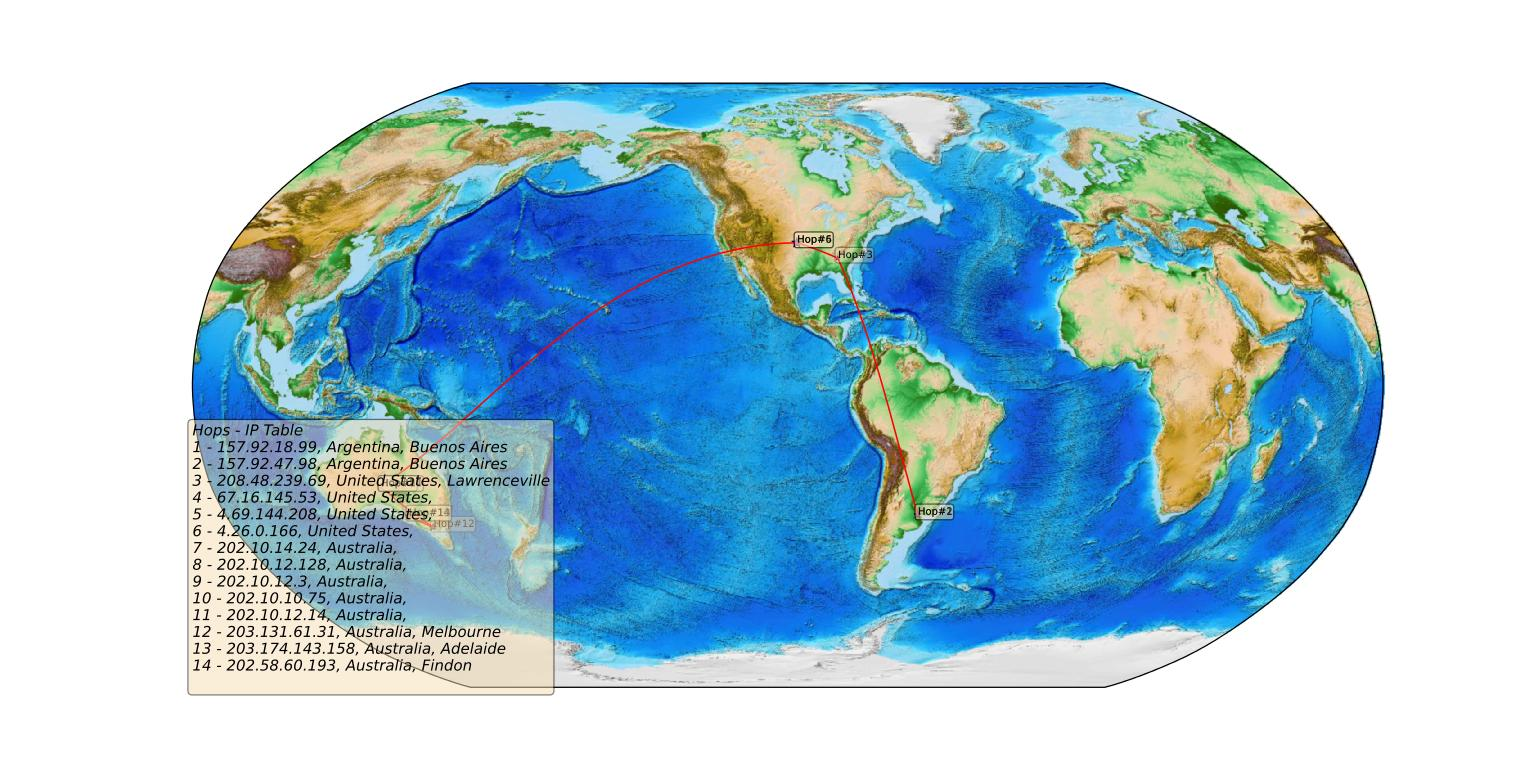
\includegraphics[scale=0.3]{../australia-experiment/figure_1.jpeg}
  \caption{Planisferio el viaje realizado por el paquete resaltado en rojo.}
	\label{fig:histo-src-sitiotrabajo}
\end{figure}

Como se puede observar se halla un salto de los Estados Unidos a Australia entre el sexto y septimo hop. Si el Z-Score cumple con su objetivo de la forma esperada, este será resaltado como un \textit{hop} de mayor importancia con respecto a los otros. Veamos que sucede con el \textit{RTT}, que es esperable aumente de manera significativa luego de este salto. El primero del siguiente par de gráficos representa el RTT entre dos host consecutivos, mientras que el segundo representa el acumulado a medida que el paquete se acerca a su destino: 

\begin{figure}[H]
  \centering	
	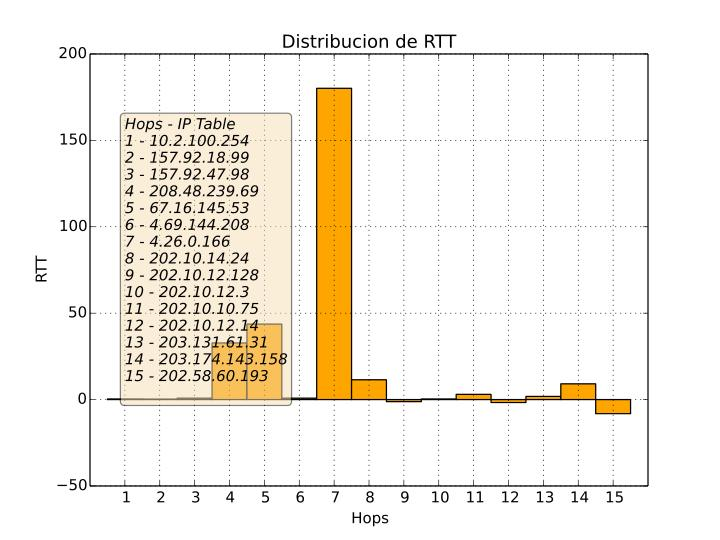
\includegraphics[scale=0.5]{../australia-experiment/bar_rtt.jpeg}
  \caption{RTT entre dos hops consecutivos medido en milisegundos.}
	\label{fig:histo-src-sitiotrabajo}
\end{figure}

\begin{figure}[H]
  \centering	
	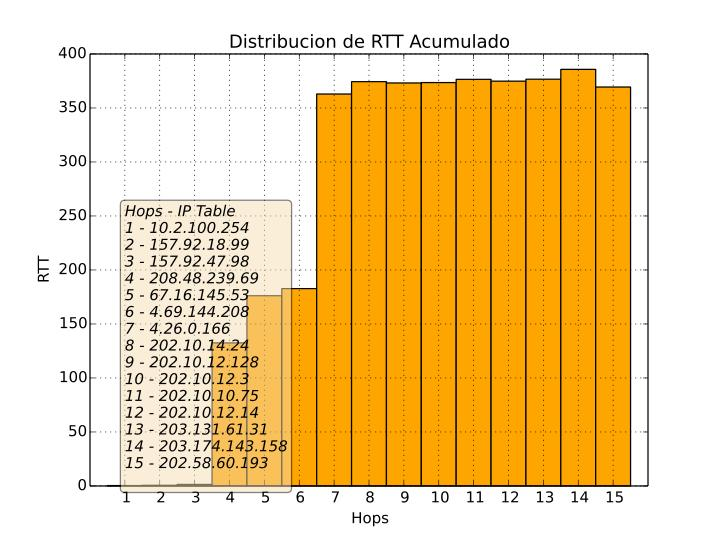
\includegraphics[scale=0.5]{../australia-experiment/bar_rtt_acum.jpeg}
  \caption{RTT acumulado del paquete a medida que avanza en su camino hacia Australia.}
	\label{fig:histo-src-sitiotrabajo}
\end{figure}

Finalmente, presentamos los resultados obtenidos con el Z-Score a partir de los valores obtenidos con la herramienta de \textit{traceroute}. Como se puede ver en el gráfico, la IP distinguida corresponde con el último nodo antes del salto transoceánico con destino a Australia. El resto de los valores o bien son negativos, o no parecen llegar a estar asociados a un nodo representativo del \textit{hop} debido a su reducido puntaje con respecto al mayor de los obtenidos. No se podría afirmar lo mismo en caso de que el puntaje entre varios de los nodos destacados hubiera sido un empate. 

\begin{figure}[H]
  \centering	
	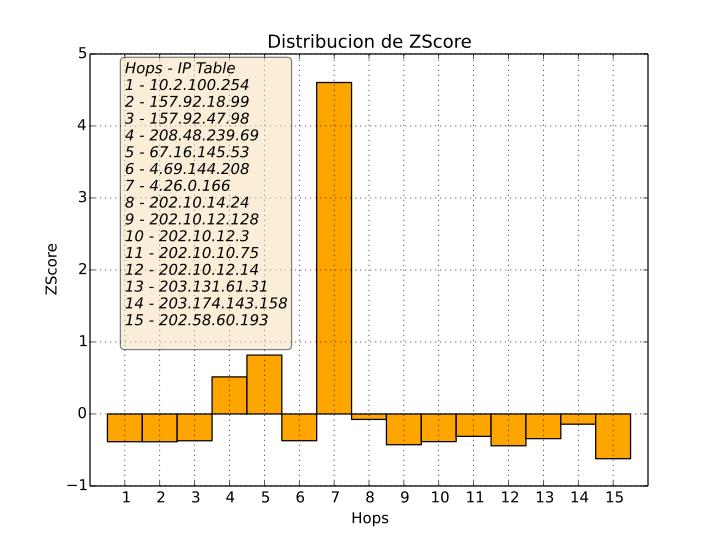
\includegraphics[scale=0.5]{../australia-experiment/bar_z_score.jpeg}
  \caption{Z-Score para cada uno de los saltos.}
	\label{fig:histo-src-sitiotrabajo}
\end{figure}

\subsubsection{Tabla de Hops de la traza}
\begin{center}
  \resizebox{\textwidth}{!}{\begin{tabular}{| c | c | c | c | c | c |}
		\hline
		Hop Score & Hop Ip & RTT Acum & RTT Incr & Hop Location & Hop Name\\
		\hline
		-0.385 & 10.2.100.254 & 0.35 & 0.35 & -,  & -\\
		\hline
		-0.386 & 157.92.18.99 & 0.63 & 0.28 & Argentina, Buenos Aires & ccc-pab2.fcen.uba.ar.\\
		\hline
		-0.372 & 157.92.47.98 & 1.43 & 0.8 & Argentina, Buenos Aires & -\\
		\hline
		0.515 & * & * & 32.758 & - & *\\
		\hline
		0.515 & * & * & 32.758 & - & *\\
		\hline
		0.515 & * & * & 32.758 & - & *\\
		\hline
		0.515 & 208.48.239.69 & 132.46 & 32.758 & United States, Lawrenceville & ethernet14-4.ar4.mia1.gblx.net.\\
		\hline
		0.818 & 67.16.145.53 & 176.14 & 43.68 & United States,  & po5.ar3.MIA2.gblx.net.\\
		\hline
		-0.371 & * & * & 0.825 & - & *\\
		\hline
		-0.371 & * & * & 0.825 & - & *\\
		\hline
		-0.371 & * & * & 0.825 & - & *\\
		\hline
		-0.371 & * & * & 0.825 & - & *\\
		\hline
		-0.371 & * & * & 0.825 & - & *\\
		\hline
		-0.371 & * & * & 0.825 & - & *\\
		\hline
		-0.371 & * & * & 0.825 & - & *\\
		\hline
		-0.371 & 4.69.144.208 & 182.74 & 0.825 & United States,  & ae-4-90.edge1.LosAngeles6.Level3.net.\\
		\hline
		4.604 & 4.26.0.166 & 362.88 & 180.14 & United States,  & AAPT-LIMITE.edge1.LosAngeles6.Level3.net.\\
		\hline
		-0.076 & 202.10.14.24 & 374.35 & 11.47 & Australia,  & po9.sclardist02.aapt.net.au.\\
		\hline
		-0.427 & 202.10.12.128 & 373.16 & -1.19 & Australia,  & te2-1-110.sclardist01.aapt.net.au.\\
		\hline
		-0.384 & 202.10.12.3 & 373.52 & 0.36 & Australia,  & bu11.sclarcore01.aapt.net.au.\\
		\hline
		-0.311 & 202.10.10.75 & 376.52 & 3 & Australia,  & bu1.mburncore01.aapt.net.au.\\
		\hline
		-0.442 & 202.10.12.14 & 374.8 & -1.72 & Australia,  & te2-2.mburndist01.aapt.net.au.\\
		\hline
		-0.343 & 203.131.61.31 & 376.63 & 1.83 & Australia, Melbourne & 1-1-1.mburninte01.aapt.net.au.\\
		\hline
		-0.142 & 203.174.143.158 & 385.73 & 9.1 & Australia, Adelaide & 203-174-143-158.ade.static-ipl.aapt.com.au.\\
		\hline
		-0.621 & * & * & -8.165 & - & *\\
		\hline
		-0.621 & 202.58.60.193 & 369.4 & -8.165 & Australia, Findon & -\\
		\hline
	\end{tabular}}
\end{center}

\subsubsection{Tabla de Hops Distinguidos}
\begin{center}
  \resizebox{\textwidth}{!}{\begin{tabular}{| c | c | c | c | c | c |}
		\hline
		Hop Score & Hop Ip & RTT Acum & RTT Incr & Hop Location & Hop Name\\
		\hline
		0.515 & *  & * & 32.758 & - & -\\
		\hline
		0.515 & *  & * & 32.758 & - & -\\
		\hline
		0.515 & *  & * & 32.758 & - & -\\
		\hline
		0.515 & 208.48.239.69 & 132.46 & 32.758 & United States, Lawrenceville  & ethernet14-4.ar4.mia1.gblx.net.\\
		\hline
		0.818 & 67.16.145.53 & 176.14 & 43.68 & United States,   & po5.ar3.MIA2.gblx.net.\\
		\hline
		4.604 & 4.26.0.166 & 362.88 & 180.14 & United States,   & AAPT-LIMITE.edge1.LosAngeles6.Level3.net.\\
		\hline
	\end{tabular}}
\end{center}

\subsubsection{Estadistica sobre las mediciones de RTT incremental}
\begin{itemize}
	\item $\overline{RTT_i}: 14.208$
	\item $STDEV(RTT_i): 36.041$
\end{itemize}

\subsubsection{Conclusion y aclaraciones}
Podemos observar que el promedio del $RTT_i$ condice con el grafico, y la desviacion estandar es alta, debido a la gran variacion del salto distinguido. En este caso particular tenemos varias aclaraciones que hacer. Para comenzar, tenemos dos resultados extraños, el primero, que el nodo distinguido marcado en el planisferio entre \texttt{157.92.47.98, Argentina, Buenos Aires} y \texttt{208.48.239.69, United States, Lawrenceville}, ve enmascarados 3 hops desconocidos, a los cuales se les calculo un RTT proporcional junto al hop de Estados Unidos. Esto no afecto la deteccion del salto entre el sur y el norte de America, pero quisimos aclararlo igualmente. Por otro lado, notemos que los saltos entre \textbf{4.69.144.208, United States, ae-4-90.edge1.LosAngeles6.Level3.net.},   \textbf{4.26.0.166, United States, AAPT-LIMITE.edge1.LosAngeles6.Level3.net.} y \textbf{202.10.14.24, Australia, po9.sclardist02.aapt.net.au.} arroja resultados extraños en la medicion del zscore. Todo parece indicar que el salto intercontinental esta entre los hosts \textbf{ae-4-90.edge1.LosAngeles6.Level3.net.} y \textbf{AAPT-LIMITE.edge1.LosAngeles6.Level3.net.} ambos ubicados en Estados Unidos, realizando una investigacion mas exhaustiva, encontramos que \texttt{AAPT Limited} es una gran compañia de telecomunicaciones de Australia, que se encarga de infraestructura, entre otras cosas, lineas submarinas. Nuestra suposicion acerca de este resultado es que el cable submarino entre \textbf{Estados Unidos} y \textbf{Australia} tiene IP de dominio estadounidense en ambos extremos del cable y el verdadero salto intercontinental se ve reflejado en el outlier del RTT incremental entre los hosts \textbf{ae-4-90.edge1.LosAngeles6.Level3.net.}, \textbf{AAPT-LIMITE.edge1.LosAngeles6.Level3.net.}.\\
Podemos ver finalmente que para este experimento, pudimos identificar los cables intercontinentales tanto con las herramientas de geolocalizacion como las herramientas estadisticas.